%META {"question":"Trong hình vuông ABCD, cạnh AB và cạnh BC có quan hệ gì với nhau?","options":["Vuông góc với nhau","Song song với nhau","Trùng nhau","Không liên quan đến nhau"],"answer":0,"note":"Hai cạnh kề của hình vuông vuông góc với nhau (ký hiệu góc vuông tại B): AB ⊥ BC."}
\documentclass[border=5pt]{standalone}
\usepackage{tkz-euclide}
% Màu dùng chung cho toàn bộ hình vẽ (ảnh stack với nền tối của web)
\definecolor{tminc}{RGB}{226,232,240}   % chữ + nét chính
\definecolor{tmblue}{RGB}{0,210,255}    % nhấn neon xanh
\definecolor{tmpink}{RGB}{255,0,200}    % nhấn neon hồng
\definecolor{tmgreen}{RGB}{0,255,136}   % nhấn neon xanh lá
\color{tminc}

\begin{document}
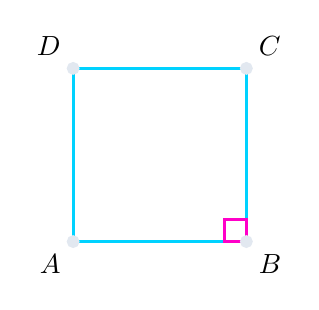
\begin{tikzpicture}[line width=1.1pt]
  \coordinate (A) at (0,0);
  \coordinate (B) at (2.2,0);
  \coordinate (C) at (2.2,2.2);
  \coordinate (D) at (0,2.2);
  \tkzDrawPolygon[tmblue,line width=1.1pt](A,B,C,D)
  \tkzMarkRightAngles[size=0.28,color=tmpink,line width=1pt](A,B,C)
  \tkzDrawPoints[size=3.5,color=tminc,fill=tminc](A,B,C,D)
  \tkzLabelPoint[below left=1pt](A){$A$}
  \tkzLabelPoint[below right=1pt](B){$B$}
  \tkzLabelPoint[above right=1pt](C){$C$}
  \tkzLabelPoint[above left=1pt](D){$D$}
\end{tikzpicture}
\end{document}
